\chapter{Simulator design} \label{simulators}

\section{RotorSim} \label{rotorsim}

% TODO this probably needs some restructuring
RotorSim \cite{brode-roger_nibriviarotorsim_2020} is a centralized simulator (see \ref{centralized-sim}) of a packet-level datacenter network model (see \ref{model}).
It is implemented in Python \cite{van_rossum_python_2009} and is single-threaded. %does python need to be cited?

\subsection{Event queue} \label{rotorsim-eventq}
\subsubsection{API} \label{rotorsim-eventq-api}

\begin{table}[ht]
\begin{center}
\label{rotorsim-eventq-api:table}
\begin{tabular}{|p{1.8in}|p{3.8in}|}\hline
\code{create(limit)} & Instantiates an event queue with the given \code{limit} \\\hline
\code{call\_at(time, event)} & Schedules \code{event} at the specified \code{time} \\\hline
\code{call\_in(delay, event)} & Schedules \code{event} at the current time+\code{delay}  \\\hline
\code{run\_next()} & Starts the event simulator, returns when \code{limit} is reached, there are no events to run, or \code{stop()} is called \\\hline
\code{stop()} & Forces the event loop to return \\\hline
\code{time} & Returns the current time \\\hline
\end{tabular}
\caption{RotorSim event queue API}
\end{center}
\end{table}

The event queue allows for the addition of new events through two functions: \code{call\_at(time, event)} and \code{call\_in(delay, event)}.
These will then appropriately add the event to the queue and return.
The exact structure of \code{time} and \code{event} are discussed in \ref{rotorsim-eventq-event}.

To event loop is started through a call to \code{run\_next()} and finishes either when there are no more events to schedule, or when it hits a limit defined at its creation.
The loop may also ended by calling \code{stop()}, breaking the loop.
Although rarely useful when running simulations to produce results, it is useful while debugging.
After being stopped, the loop may be resumed through another call to \code{run\_next()}.

% wow is this section badly written
In order to make code more readable, and less error-prone, the module also exports a function decorator, \code{@delay(amount)} that will wrap a function in a call.
A useful case for this is to enforce delays in reconfiguration or receiving packets.
For example, if an switch $S$ has a \code{recv(packet)} function that processes incoming packets, it may be useful to wrap this with a \code{@delay(latency)}, enforcing that anyone calling the function waits an additional $latency$ amount.
Calling \code{S.recv(packet)} then doesn't actually call the function itself, but schedules an event $latency$ later that will call said function.
In practice, most calls are made this way, clearing the code of many \code{call\_in} statements.


% TODO write up full example?


\subsubsection{Event structure} \label{rotorsim-eventq-event}
RotorSim's event queue is implemented using Python's \code{heapq} \cite{noauthor_heapq_nodate}.

Python tuples are ordered by comparing the first element of the tuple, going to the next in case of a tie.
This naturally leads to events being a tuple of time and event description.

Python allows for the treatment of functions as values, as well as for calling a function with an array, or a dictionary as arguments through the \code{*args} and \code{**kwargs} idioms.
Once the

In addition to \code{(time, function, args, kwargs)}, the event queue adds a user-controlled priority value to allow for the breaking of ties for events that happen simultaneously.
Although this isn't strictly required, it does simplify simulator design around configuration changes.
For example, if the routing table of a device changes and a packet sent, both at time 100, it is often intended that the configuration change take place before the packet is routed, avoiding odd situations where a packet is routed along a path that no longer exists.

Finally, as suggested in \code{heapq}'s documentation, there is a final integer, a counter, inserted after the priority. Ostensibly this breaks ties between events having the same time and priority by the order in which they are inserted.
This property is not used in the simulator, however it stops python from 

Each event is a tuple consisting of, in order, the current time, a priority (lower means run earlier), a unique counter, 



\subsection{Limits} \label{rotorsim-limits}

There were two main frustrations with RotorSim, its large memory usage and "slow" performance.

\paragraph{Memory usage} \label{rotorsim-mem}
Large simulations used up a lot of memory.
Part of this is due to the large amounts of objects being actively used, see \ref{limits-mem}, but Python also offers little to no control of the underlying memory representations of objects.
%TODO more
%TODO numbers

\paragraph{Low performance} \label{rotorsim-perf}
In addition to large memory usage, it often took over 24h, sometimes even up to 72, to get results.
This significantly slows down the research iterations.
Although this was sometimes mitigated thanks to being able to run hundreds of simulations simultaneously, this was only interesting when we wanted to explore a large cross-section of different parameters.
%TODO more
%TODO numbers



\subsection{Runtime} \label{rotorsim-runtime}

Different interpreters exist for the python programming language, the default being CPython.
However, I found that using PyPy \cite{team_pypy_2019} yields an almost 2x performance improvement for the simulator compared to CPython.
Even Pypy can run virtually all Python code, numpy \cite{van_der_walt_numpy_2011} is difficult to set up properly.
For RotorSim, numpy was only used for some random number generation, making moving away from the package easy.









\section{Rustasim} \label{rustasim}

Rustasim \cite{brode-roger_nibriviarustasim_2020} is a parallel discrete event simulator implemented in Rust \cite{klabnik_rust_2018}\cite{matsakis_rust_2014}, and heavily benefiting from the well-optimized data structures of the crossbeam library \cite{noauthor_crossbeam-rscrossbeam_2020}.

The main impetus for exploring a different programming language came from repeatedly hitting memory limits with RotorSim (even with 96GB of RAM!) and being frustrated at its slow speed.
A goal was proposed to make a simulator run medium-sized simulations within a few hours, yielding an objective of managing to simulate 100Gb worth of traffic moving for every wall-clock second the simulator is run.
For context, Rotorsim was able to move TKGbps. %TODO get number


\subsection{Language choice} \label{rustasim-language}

In order to achieve the desired goal, I decided to re-evaluate the choice of programming language.
Rotorsim used Python because it was chosen for a class project, which later turned into a research simulator.
There was no formal evaluation of that choice.

The evaluation criteria were a combination of resulting speed and ease of development.
The candidate languages were: Python, Go \cite{donovan_go_2015}, C \cite{kernighan_c_1988}, and Rust.
All but Rust were chosen due to my familiarity with them, Rust chosen because recommended to me.
Go was interesting due to potential for easy concurrency and parallelism.
C was chosen for its reputation as a high-performance language.

For each of the languages I implemented a simple simulator consisting of one device with a `loopback' link, a connection feeding right back to itself after a small latency.
The goal was simply to see how fast the simulator was able to be pushed, and how easy or not developping in the language was.
\begin{itemize}
\item Python took a few hours to re-implement, and was able to move 25Gb of traffic for every second of realtime on the link.

\item Go took almost a day, due to not having a generic function structure such as python, eventually solved through the use of closures.
However the performance was, surprisingly, nearly identical to python's at around 25Gbps on the same machine.
Attempts to make the simulation parallel, by processing the event and heap operations in parallel slowed down the simulator due to the need for synchronization between the different routines.

\item Rust took much longer to develop, around 4-5 days, most of which was spent getting familiar with a new memory management model.
Rust also does not take well to functions whose type is not defined at compile time.
However, Rust has structured enumerations, allowing all the different event types to be defined at compile time. %TODO check name
The event loop could then, on a pre-defined event, call a specific function.
Since the different enumeration variants can also carry distinct data, the arguments for the function can be carried with the variant, allowing flexibility in the types of functions called.
After some quick optimizations, Rust moved 125Gb per second, faster than goal.

\item The C implementation never took off, the library management system being difficult to manage, simple data structures like the heap requiring re-implementation.
\end{itemize}

Thus Rust became the top choice, despite a long implementation time, since I believed this was due to the initial learning cost, and not to a fundamental feature of the language.
In addition to switching to Rust, significant effort was put into parallelizing the simulation.
After having spent significant time developing the full simulator, that bet has proven correct, the language is very rarely what is holding development back.



\subsection{System overview} \label{rustasim-overview}

%TODO use newer version
\begin{figure}[h]
\centering
\label{rustasim-overview:fig}
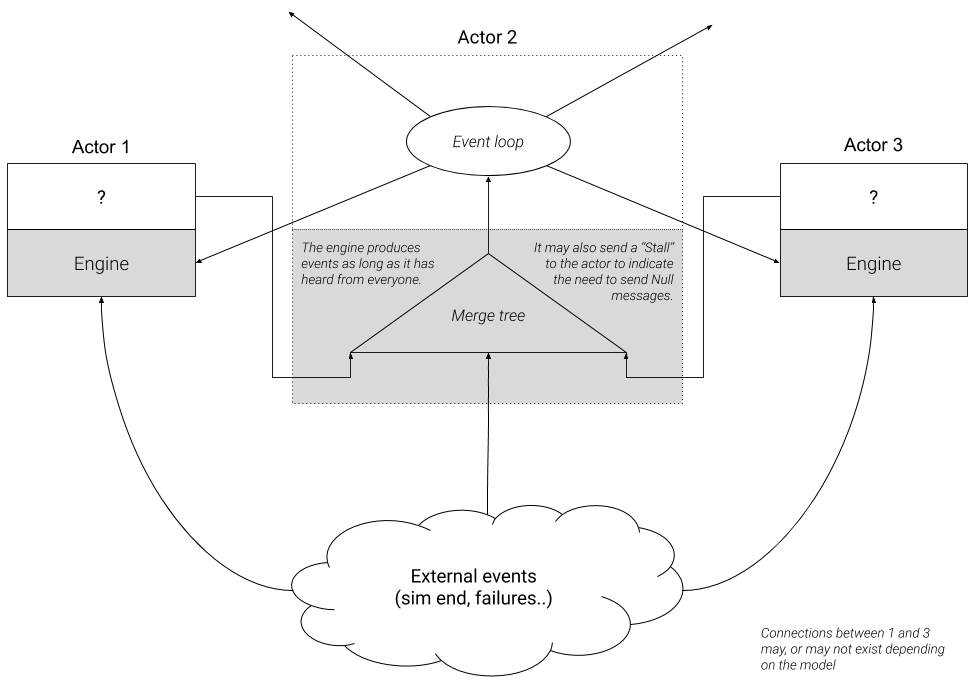
\includegraphics[width=\textwidth]{rustasim-overview}
\caption{Rustasim system diagram (TODO pretty diagram)}
\end{figure}

A Rustasim simulation consists of many actors, each running concurrently, not necessarily simultaneously, to all others.
This concurrency brings with it all the challenges described in section\ \ref{pdes}: preserving causality and guaranteeing progress.

To make developing models easier, Rustasim enforces a separation between the model and the code that deals with the parallel aspects of the simulation, the `engine'.
The engine and the model then have a application/system relationship: the engine receives all incoming events, arranges them in order and detects stall, returning to the user/model the events in order.
This is abstraction very similar to how applications interface with TCP: the application receives the bytes in-order while the OS handles the complexities of re-ordering and managing the connection.
The actor receives the events in order through an iterator, matches on the event type and executes the appropriate action.
It is required to take certain actions upon receiving certain events

Since there may be thousands or more of actors, it is not possible to spin up separate threads for each of them.
Instead Rustasim spins up as many worker threads as there are available cores, and actors are scheduled on the workers.
The details of the scheduling are described in \ref{rustasim-sched}.



\subsubsection{The actor-engine abstraction} \label{rustasim-actor-engine}

The events in a distributed simulation are slightly more complex than in a centralized one.
Although most events processed by actors, are still model events, there is a need for additional event types in order to guarantee progress.\\
\code{Null} events are required to signal neighbours that it is safe for them to progress up to a certain time without waiting for this actor.
Without these messages, an actor cannot be sure if the silence from the neighbour comes from a lack of events to send, or from a delay in computation.
Although \code{Null} events are required to guarantee progress, actors will never receive them: they are only useful for the engine to progress, the actor need not take action on them.
The sole purpose of \code{Null} events is to allow the neighbours' engines to make progress.\\
Because the \code{Null} events require model-level knowledge to send, the engine cannot do so on its own.
However, it is the engine that will become aware of a potential deadlock, not the actor.
Therefore, to inform the actor of a potential stall, the engine generates a \code{Stalled} event.
Upon receiving such an event, the actor is \emph{required} to send all necessary neighbours a \code{Null} event updating how far they may progress.
If a neighbour has already received another event at, or past, the time the \code{Null} event would be received, the \code{Null} event is not sent.\\ %TODO make clearer
Finally, \code{Close} events tell the actor to return from its event loop.
Although this might seem trivial, it does require a little care, it is easy to leave the simulation hanging at this point.
It is necessary to also inform neighbours that we have no more events to communicate to them.
This can be done by sending \code{Null} events that pass closing times, or by sending \code{Close} events to the neighbours.
This imp

% TODO re-write, more details, reorgnize, cite?
\paragraph{Compiler enforcement}
The modularity between the actor and the engine is strictly enforced by the Rust compiler.
The events the engine deals with are parametrized through a generic type \code{T} representing the model events.
Because the engine code is generic over \code{T}, it cannot make any assumptions about what the type looks like, lest the Rust compiler errors.
However, when compiled, the compiler will fill in the type appropriately and is able to optimize as though the type were written explicitly written in.\\
This separation between the model and the engine also allows for many different models to be implemented using the same engine, allowing for significant reuse between projects.
This is particularly appealing because most optimizations are implemented in the engine itself, and allowing further optimizations to be propagated to many simulations.
This separation also allows the writing of tests for the engine using a trivial model, making it easier to validate the engine and catch subtle errors.

\subsection{Indexing} \label{rustasim-indexing}

Although most code consider the performance cost of a hash to be negligible, at the scale of TKTK, it becomes noticeable.
There is therefore a large incentive to not use hash tables and rely on the significantly faster direct indexing offered by arrays.
However, most data structures maintained by both the actor require indexing by the neighbour's \code{id}.
This \code{id} is unique across all actors and is useful for routing and for keeping track of who an event's sender is.

An alternative to structuring these data by \code{id} is to add every neighbour to an array and refer to them by their index.
Unfortunately that mapping isn't going to be regular across all actors, and some structure still explicitly require an \code{id}, notably packet destinations.

In order to minimize the amount of hashes to be made, each actor keeps track of a single hash table that maintains a translation from \code{ids} to an index \code{ix}, as well as an array containing an \code{ix} to \code{id} translation, mostly used for debugging purposes.
In addition, if the \code{id}s of all the devices in the network are continuous starting from 0, the routing table can be indexed, not hashed, by \code{id}, and return the appropriate index.

However, it is possible to avoid hash table lookups entirely with the cooperation of the engine.
The engine doesn't care about the model \code{id} of its neighbours, it only needs to receive its events.
By having the engine maintain the incoming queues in an array the same order as the actor has setup its \code{id}s, it is possible to translate the source \code{id} of the event to an index without needing a lookup.
Indeed, hen the engine removes an event from a queue, it necessarily knows the index of that queue in its array of incoming queues.
It can then overwrite the incoming event's source field with the appropriate index, no lookup required.

% TODO there is no section where you talk about servers, should go in the model chapter too
The only exception to the lack of hashtables is the list of flows at a server.
Flows are uniquely identified by a global id and servers maintain a mapping from \code{flow\_id} to the appropriate flow receiver.
However, this can probably be optimized out and profiling has not revealed it as a bottleneck.

The combination of these optimizations mean that there is almost no need to execute a hash table lookup in the normal processing of events.
The full translation tables, although never used in a proper simulation run, can be extremely helpful in debugging.

%\subsection{Data structures} \label{rustasim-data-structure}
\subsection{Message passing} \label{rustasim-message-passing}
SPSC


\subsection{Multi-queue merging} \label{rusatim-tree}

This is the core of the engine: merging multiple queues together, and returning the next event if it has heard from all neighbours, as described in \ref{null-messages}.
If a neighbour has not been heard from, the scheduler should return a \code{Stalled} event.

\subsubsection{An initial approach: heaps}
An initial approach might be to maintain a heap of all received event along with a counter for the number of events in the heap from each sender.
The running time for this structure is sub-optimal, since it grows with to the amount of events in the queue, which is, due to the nature of waiting on everyone, always going to be nearly equal to, or greater than the number of neighbours.
The algorithmic complexity of processing or returning an event is then $O(\log e)$, with $e$ being the number of events in the queue.

An improved approach would take only the top event from each of the senders and maintain a heap of those.
The heap is then bounded by the number of senders, and the book-keeping is reduced to whether or not a sender has an element in the heap.
This structure then has an algorithmic complexity of $O\left(\log n\right)$
This works relatively well and supports somewhat fast running times. %TODO numbers plz!

% TODO expand on structure more: state goes between waiting and continuously popping

Processing happens in two stages... is that fundamentally true?

\subsubsection{Loser trees}

Although there does not exist to my knowledge a structure with a better algorithmic performance, there exists structures with significantly better constant factors.
Notably, this problem is essentially identical to the problem of merging tapes: the reader, either tape head or channel consumer, cannot look ahead in the data, and we are allowed to assume the data already sorted.
Tournament trees in particular solve this problem elegantly.

A tournament tree takes in a certain number of elements to compare, here the next element of each of the queues and pairs them off.
The winner of each exchange, the event to be scheduled the soonest, moves on to fight another winner.
This process eventually forms a tree analogous to the structure of many tournaments.
Although it may be natural to record the winner of each exchange, recording the looser makes for a significantly more elegant algorithm as described by Knuth \cite{knuth_art_1998}.

% Describe the loser tree process

\paragraph{Dealing with ties}

\subsection{Scheduling} \label{rustasim-sched}

In the rare cases where there are less actors than available cores and there isn't contention on the system (no other CPU heavy job), it is possible to give each actor its own thread.
In the case where an actor stalls and is waiting on another, it can `busy-wait', burning CPU cycles until there is a new event on the channel.
More subtle synchronization primitives could be used, but they have some overhead, whereas checking in a tight loop has none.

However, The huge disadvantage of busy-waiting is that it gives the operating system no help as to which thread should be scheduled next, often scheduling threads that have nothing to do but burn cycles.
This issue alone is enough to make the simulator over 1,000x slower. %vrify + experiment?
Explicitly yielding the thread on a stall improves the situation, but not much, since the OS still has no clear idea of who is best to schedule next. %numbers plz
In fact, cursory experiments suggest that it often repeatedly picks the same threads to schedule, letting it advance ahead of the rest, stall, and get rescheduled soon after, making little progress before stalling again, and so on.
Unfortunately switching between threads is an expensive operation for the operating system, and can easily take up a huge fraction of the simulation time.
In some runs, this process took up almost two thirds of the simulation time, i.e. removing the scheduling issue could speed up the simulation by a factor of 3. %experiment, plz
In addition to the overhead of thread switching, repeatedly stalling an operation sends out more \code{Null} events than necessary: they were not sent because of a deadlock, but because of a scheduling issue, creating overhead.
On its own, sending more events may not seem like a big issue, but these \code{Null} events can become the main thing the stragglers receive, sometimes the fraction of \code{Null} events exceeding TK\%. %experiment

However, a better setup would be to advance an actor until it stalls and sends \code{Null} events, stop it, schedule every other actor, and then come back.
This pattern guarantees that our actor is now last, or at least near it, before scheduling it again.
Straggling behind everyone means that it can run for longer: enough to catch up, and then enough until it stalls.

This is essentially a form of round-robin.
TK

\subsubsection{Work stealing}

Work stealing good, fast
problem is can't distribute without central
problem with central is tooooo slowwww

instead steal from neighbour in ring
still too slow

how about a ring of messages
traffic jams
ring+steal
happiness :)